\documentclass[russian,utf8,nocolumnxxxi,nocolumnxxxii]{eskdtext}
\usepackage[T1,T2A]{fontenc}
\usepackage[utf8]{inputenc}
\usepackage{graphicx}
\graphicspath{{pictures/}}
\usepackage{pgfplots}
\pgfplotsset{compat=1.9}%%%%%%%%%%%%%
%\usepackage[english,russian]{babel}
\usepackage{amssymb,amsmath}
\usepackage{tikz}
\usepackage{siunitx}
\usepackage{nccmath}

\usepackage[american,cuteinductors,smartlabels]{circuitikz}
\usepackage[backend=biber]{biblatex}
\addbibresource{error_estimation_otchet.bib}
\usepackage[]{hyperref}
\hypersetup{colorlinks=true,}
\usepackage{textcomp}
\usepackage{float}
\newcommand{\No}{\textnumero}
\ESKDdepartment{Федеральное агентство по образованию}
\ESKDcompany{Санкт-Петербургский государственный электротехнический университет "ЛЭТИ"}
\ESKDtitle{Пояснительная записка к Курсовой работе}


\ESKDsignature{Вариант N22}
\ESKDauthor{ПрокудинБ.С.}%%%%%%%%%%
\ESKDchecker{ПрокшинА.Н.}%%%%%%%%%%
\ESKDdocName{по дисциплине "Информатика"}

\begin{document}
\maketitle

\newpage

\tableofcontents%  содержание,атоматическое

\newpage % С новой страницы

\section{Введение} % Пункт с автонумерацией

\subsection{Цель курсовой работы} % Подпункт с автонумерацией

Уметь применять персональный компьютер и математические пакеты прикладных программ в инженерной деятельности.

\subsection{Тема курсовой работы:}

Решение математических задач с использованием математического пакета "Scilab" или "Reduce-algebra".

\subsection{Содержание курсовой работы курсовой работы:}

\begin{enumerate}
%%%%%%%%%%%%%%%%%%%1111111111
\item Даны функции $f(x)=\sqrt{3}sin(x)+cos(x)$ и $g(x)=cos(2x+\frac{\pi}{3})-1$
\begin{itemize}
  \item Решить уравнение f(x)=g(x)
  \item Исследовать функцию h(x)=f(x)-g(x) на промежутке $[0;\frac{5\pi}{6}]$
\end{itemize}
%%%%%%%%%%%%%%%%222222222222222222
\item Найти коэффициенты кубического сплайна, интерполирующего данные, представленные в векторах $V_x$ и $V_y$. С каординатами  0; 1,25; 2; 2,625; 4,25 по оси абсцисс и 3; 2,925; 3,75; 3,72; 4,444 по оси ординат.% Переписать

Построить на графике функцию f(x), полученную после нахождения коэффициентов кубического сплайна.

Представить графическое изображение результатов интерполяции исходных данных различными методами с использованием встроенных функций.
%%%%%%%%%%%%%%%%%%%%%%%%3333333333333333
\item Решить задачу оптимального распределения неоднородных ресурсов. На предприятии постоянно возникают задачи определения оптимального плана производства продукции при наличии конкретных ресурсов (сырья, полуфабрикатов, оборудования, финансов, рабочей силы и др.) или проблемы оптимизации распределения неоднородных ресурсов на производстве.
\\Пусть в распоряжении завода железобетонных изделий (ЖБИ) имеется m видов сырья (песок, щебень, цемент) в обёмах $a_i$. Требуется произвести продукцию n видов. Дана трёхнологическая норма $c_{ij}$ потребления отдельного i-го вида. Известна прибыль $П_i$, получаемая от выпуска единицы продукции j-го вида. Требуется определить, какую продукциюи  в каком количестве должен производить завод ЖБИ, чтобы получить максимальную прибыль.
\end{enumerate}
%%%
\begin{table}[h]
%\renewcommand{\arraystretch}{1.8} % всех высота строк
%\renewcommand{\tabcolsep}{0.15cm} % отступ от текста до линии разметки таблицы
\caption{\label{TRT1} Задание согласно варианту:  }
\renewcommand{\tabcolsep}{0.5cm}
\begin{center}
\begin{tabular}{|c|c|c|c|c|c|c|c|c|c|c|c|}
\hline % начертить горизонтальную линию.
Используемые ресурсы &\multicolumn{4}{|c|}{Изготавливаемые изделия} & Наличие\\
ресурсы $a_i$ & $U_1$ & $U_2$ & $U_3$ & $U_4$ & ресурсов $a_i$\\

\hline
  %\renewcommand{\tabcolsep}{5cm} % отступ от текста до линии разметки таблицы
  Песок          & 3  & 7  & 6  & 7  & 16  \\
  Щебень         & 4  & 5  & 5  & 1  & 12  \\
  Цемент         & 4  & 4  & 9  & 8  & 35  \\
  Прибыль, П$_j$ & 35 & 45 & 36 & 28 &   \\
 \hline
\end{tabular}
\end{center}
\end{table} 

%%%%%%%%%%%%%%%%%%%%%%%%%%%%
%%%%%%%%%%%%%%%%%%%%%%%%%%%%%%

\newpage

%%%%%%%%%%%%%%%%%%%%%%%%%%%%%%



\section{Исследование функции.}
%%%%%%%%%%%%%%%%%%%%%%%%%%%%%%
\normalsize Даны функции $f(x)=\sqrt{3}sin(x)+cos(x)$ и $g(x)=cos(2x+\frac{\pi}{3})-1$
\begin{itemize}
  \item Решить уравнение $f(x)=g(x)$
  \item Исследовать функцию $h(x)=f(x)-g(x)$ на промежутке $[0;\frac{5\pi}{6}]$
\end{itemize}
\par
\normalsize Решение уравнения и исследование функции проводиться при помощи программы "Scilab", для удобства написания и корректировки вводимых формул исполизуется встроенный в программу текстовый редактор SciNotes, позволяющий записывать скрипты, с которыми можно вести работу в командном окне.


\subsection{Решение уравнения $f(x)=g(x)$}

\normalsize  Рассмотрим функции $f(x)=\sqrt{3}(x)+cos(x)$ и $g(x)=cos(2x+\frac{\pi}{3})-1$ 
В программе "Scilab" создадим скрипт (Рис. 1), в который запишем обе функции и выведем их в одном графике (Рис. 2).
Чтобы узнать решения уравнения $f(x)=g(x)$ нужно найти нули функции $h(x)=\sqrt{3}sin(x)+cos(x)-cos(2x+\frac{\pi}{3})+1$ , но в программу "Scilab" вводить эту функцию не имеет смысла т.к. программа сама ввведет её из имеющихся в условии.
Сразу можно педположить что у функции $f(x)=\sqrt{3}(x)+cos(x)$ период равен $2\pi$ а у $g(x)=cos(2x+\frac{\pi}{3})-1$ период равен одному $\pi$ \\ Тогда, т.к.периоды обеих функций кратны.У функции он будет $h(x)=\sqrt{3}sin(x)+cos(x)-cos(2x+\frac{\pi}{3})+1$ будет равен $2\pi$ 
 
 
\normalsize Чтобы найти корни уравнения $f(x)-g(x)=0$ воспользыемся функцией fsolve.Для этого нужно ввести примерные значения функции в виде вектора,  fsolve будет находить ближайшие решения.

Из графика функции (Рис.2) видно что у функций имеется не ясно является ли точка х2 точкой косания, иле же функция проходит через ноль, и хоть из функции понятно что точка х2 является точкой касания, ещё раз убедимся в этом, задав в векторе примерных значений зададим две точки, стоящие справа и слева от точки х2.
Так же для того чтобы убедиться, что период функции равен $2\pi$ найдём точку четвёртого пересечения х4, и если $x4=x2+2\pi$ то период действительно равен $2\pi$
Так же для нахождения более првычных нам значений разделим полученные ответы на $\pi$
%%%%%%%%%%%%%%%%%%%%%%%%%%%%
\begin{figure}[H]
\center{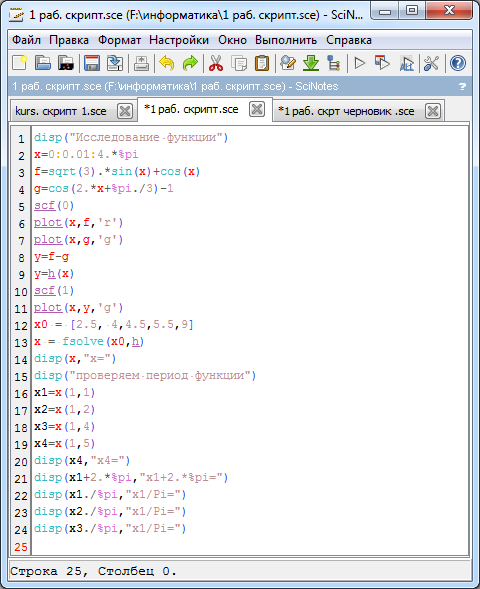
\includegraphics[width=0.9\linewidth]{1,1.png}} \\
\caption{Скрипт в текстовом редакторе SciNotes}
\end{figure}

\begin{figure}[H]
\center{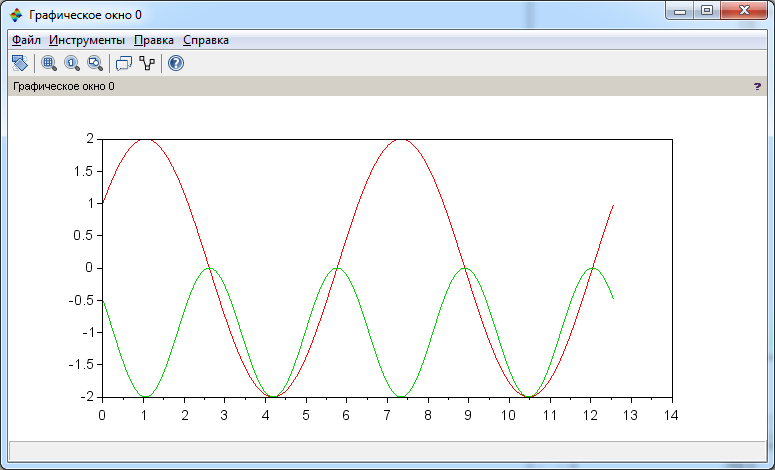
\includegraphics[width=0.8\linewidth]{1,2.png}} \\
\caption{графики функций $f(x)=\sqrt{3}sin(x)+cos(x)$ и $g(x)=cos(2x+\frac{\pi}{3})-1$}
\end{figure}

\begin{figure}[H]
\center{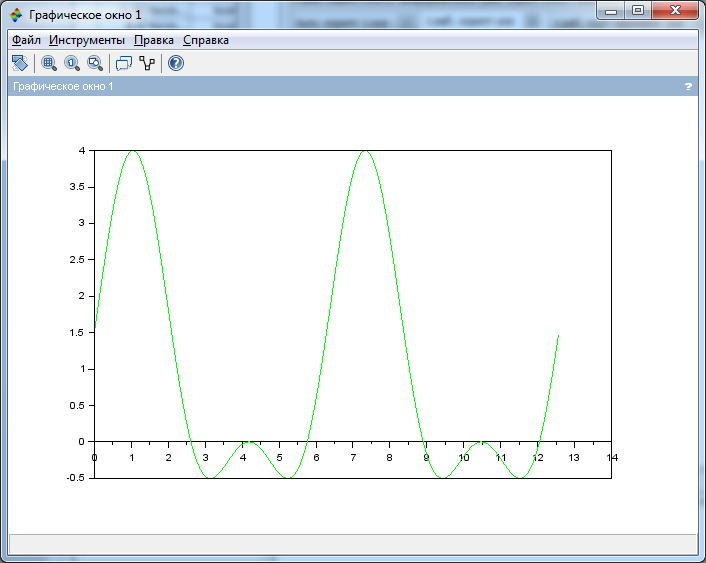
\includegraphics[width=0.8\linewidth]{1,3.png}} \\
\caption{график функции $h(x)=\sqrt{3}sin(x)+cos(x)-cos(2x+\frac{\pi}{3})+1$}
\end{figure}

\begin{figure}[H]
\center{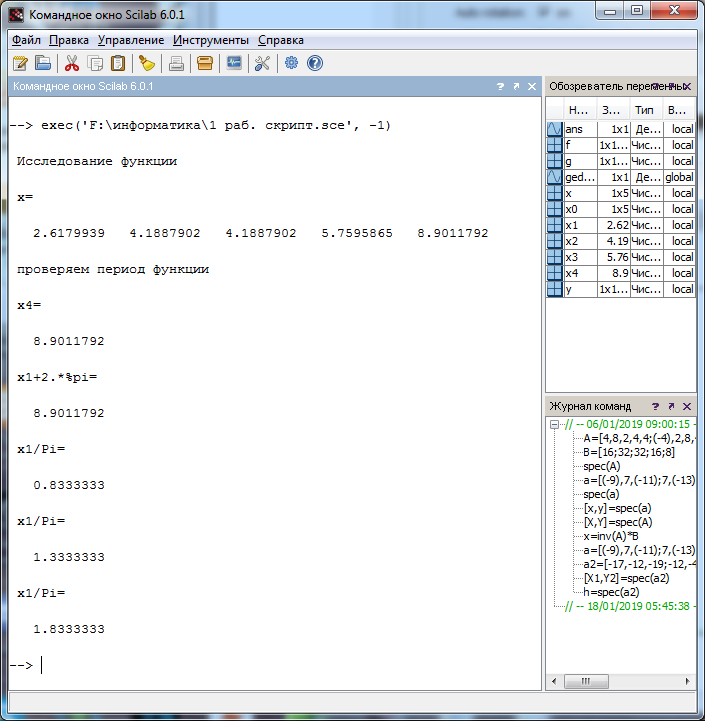
\includegraphics[width=0.8\linewidth]{1,4.png}} \\
\caption{команное окно с вычисленными по скрипту значениями}
\end{figure}

%%%%%%%%%%%%%%%%%%%%%%%%%%%%%

\normalsize В результате вычислений мы получили 5 результатов вычислений при которых функция $h(x)=\sqrt{3}sin(x)+cos(x)-cos(2x+\frac{\pi}{3})+1$ равна нулю при х равном:
2.6179939 4.1887902 4.1887902 5.759865 8.9011792 Но второй и третий результаты -- это одна и та же точка, что доказывает что функции $f(x)=\sqrt{3}sin(x)+cos(x)$ и $g(x)=cos(2x+\frac{\pi}{3})-1$ касаються друг друга, но не пересекаются.
Поэтому получаем ответы:
$$X_1=2.6179939$$
$$X_2=4.1887902$$
$$X_3=5.759865$$
$$X_4=8.9011792$$

\normalsize Период функции равен $2\pi$ т.к. $X_2+2\pi=X_4$. Данное равенство являеться доказательством, сам период был ранее установлен аналитически.
\par
В результате вычислений и упрощений ответов найдены решения уравнения  $f(x)=g(x)$ от функций $f(x)=\sqrt{3}sin(x)+cos(x)$ и $g(x)=cos(2x+\frac{\pi}{3})-1$:
\par
$$x_1=\frac{5}{6}\pi+2n\pi,n\in Z$$
$$x_2=\frac{8}{6}\pi+2n\pi,n\in Z$$
$$x_3=\frac{11}{6}\pi+2n\pi,n\in Z$$







%%%%%%%%%%%%%%%%%%%%%%%%%%%%%%%%%%%%%%%%%%%%%%%%%%%%%%%%%%%%%%%%%%%%%%%%%%%%%%%%%%%%%
\subsection{Исследование функции $h(x)=f(x)-g(x)$ на промежутке $[0;\frac{5\pi}{6}]$}
%%%%%%%%%%%%%%%%%%%%%%%%%%%%%%%%%%%%%%%%%%%%%%%%%%%%%%%%%%%%%%%%%%%%%%%%%%%%%%%%%%%%%


\begin{figure}[H]
\begin{tikzpicture} [scale=2]
\draw[thin, ->] (0,0) -- (4.5,0) node[below] {$X$};
\draw[thin, ->] (0,0) node[below] {$0$} -- (0,5) node[left] {$Y$};
\draw[domain=0:(5*3.14)/6,  blue] plot ({\x},{sqrt(3)*sin(\x r)+cos(\x r)-cos(\x*2 r + pi/3 r)+1}) node[below, black] {$\frac{5}{6}\pi$};
\end{tikzpicture}
\caption{ функция h(x)=f(x)-g(x) на промежутке $[0;\frac{5}{6}\pi]$}
\end{figure}


1. Пересечение функции с осью Х \\
Функция пересекает ось Х в точке $(\frac{5}{6}\pi,0)$ \\


2. Пересечение функции с осью Y \\
$x=0$ \\
$y_{(x0)}=sqrt(3)*sin(0)+cos(0)-cos(0 + pi/3)+1=0+1-0,5+1=1,5$ \\


3. Найдём экстремум функции
 Найдём экстремум Функции подбором  через её первую производную. В "Scilab" за это отвечает встроенная функция \\*
 numberivative.
\\ \\
\begin{figure}[H]
\center{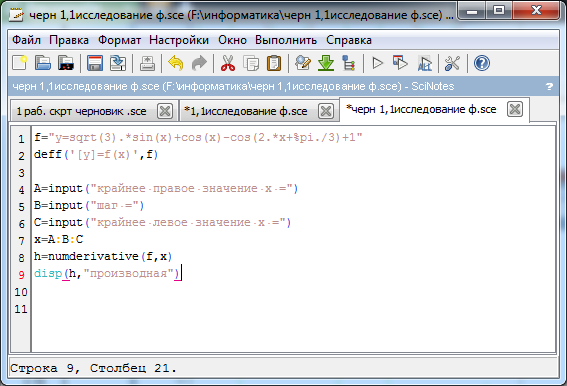
\includegraphics[width=0.8\linewidth]{1,6.png}} \\
\caption{Скрипт для подбора нулей производной}
\end{figure}

\begin{figure}[H]
\center{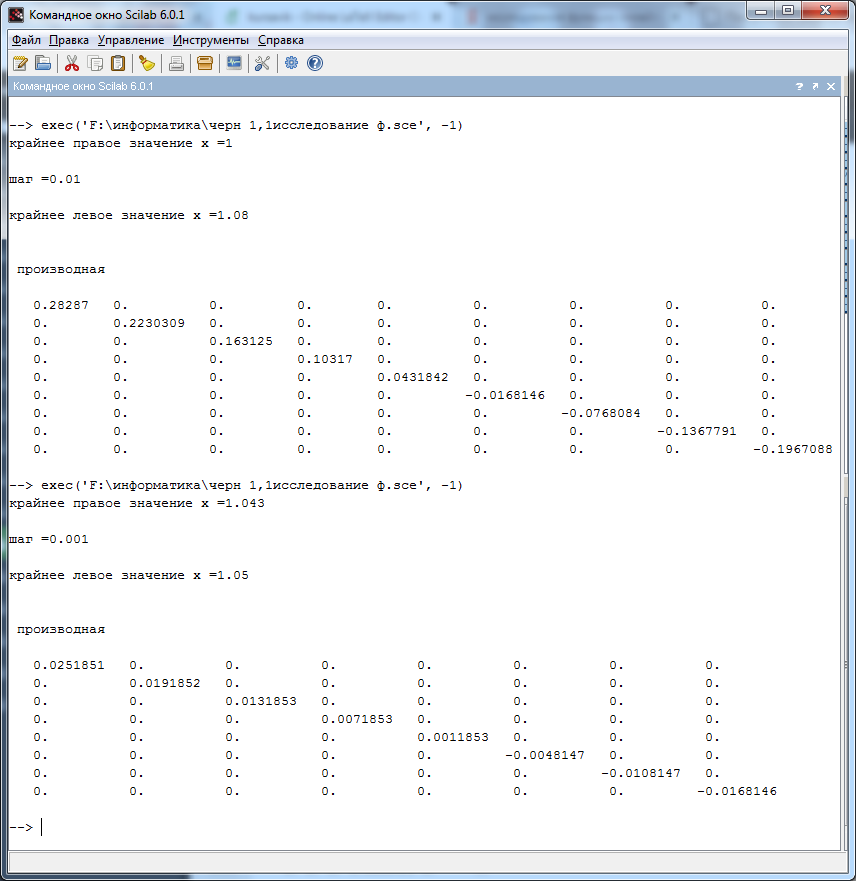
\includegraphics[width=0.8\linewidth]{1,7.png}} \\
\caption{Нахождение точки максимума в командном окне}
\end{figure}
 

Из ряда значений видно, что ноль производной находиться где-то между точками (1.047,0) и (1.048)
Но принимая во внимание то что нашу функцию можно разложить на две более простые синусоидальные функции $f(x)=\sqrt{3}sin(x)+cos(x)$ и $g(x)=cos(2x+\frac{\pi}{3})-1$, несложно заметить, что у них нет относительного смещения по оси х и поэтому сопоставив графики становиться понятно, что точка максимума должна находиться на $(\frac{1}{2}\pi,0)$
левее нуля саной функции.
$$ \left(\frac{5}{6}-\frac{1}{2} \right)\pi=\frac{1}{3}\pi$$
Что совпадает с нашим приблизительным ответом, полученным в "Scilab" \\
 Экстремум функции в точке $(\frac{1}{3}\pi,4)$ \\

 4. Функция $h(x)=\sqrt{3}sin(x)+cos(x)-cos(2x+\frac{\pi}{3})+1$ не может иметь асимптот т.к. является синусоидальной. \\
 
 5. Функция $h(x)=\sqrt{3}sin(x)+cos(x)-cos(2x+\frac{\pi}{3})+1$ не имеет разрывов \\
 
 6. Функция $h(x)=\sqrt{3}sin(x)+cos(x)-cos(2x+\frac{\pi}{3})+1$ возростает на промежутке $(0,\frac{1}{3}\pi)$ и убывает на промежутке$(\frac{1}{3}\pi,\frac{5}{6}\pi)$
 













\newpage


%%%%%%%%%%%%%%%%%%%%%%%%%%%%%%%%%%%%%%%%%%%
\section{Исследование кубического сплайна.}
%%%%%%%%%%%%%%%%%%%%%%%%%%%%%%%%%%%%%%%%%%%
 Найти коэффициенты кубического сплайна, интерполирующего данные, представленные в векторах:\\
$$V_{x}=[0,1.25,2,2.625,4.25]$$ 
$$V_{y}=[3,2.925,3.75,3.72,4.444]$$
Построить на графике функции $f(x)$,полученную после нахождения коэффициентов кубического сплайна. 
\\Оценить погрешность интерполяции в точке $x=3.1$. Вычеслить значение функции в точке $x=2.1$.
\\Представить графическое изображение результатов интерполяции исходных данных различными методами с использованием встроенных функций\\ splin(x,y,“natural”), splin(x,y,“clamped”), splin(x,y,“not\_a\_knot”), splin(x,y, “fast”), splin(x,y,“monotone”), interp(xx,x,y,d)

\subsection{Нахождение коэффицентов кубического сплайна}

\normalsize Найдем уравнение сплайна проходящего через пять точкек $(x_1, y_1),\\
(x_2, y_2), (x_3, y_3), (x_4, y_4), (x_5, y_5) $. Для того чтобы потенциальная энергия изогнутой
металлической линейки(сплайна) принимала минимальное значение,
производная четвертого порядка должна быть равна нулю, значит мы
можем представить сплайн полиномом третьей степени на каждом отрезке
$[x_i, x_{i+1}]$
$$F_i(x) = A_{i0} + A_{i1}x + A_{i2}x^2 + A_{i3}x^3, где x \in [x_i, x_{i+1}]$$

Найдём коэффиценты $A_{ij}$ исходя из того, что изгиб функции слева и справа совпадает. На каждом из отрезков $[x_i,x_{i+1}]$ график $F_i(x)$ проходит через точки $y_i,y_{i+1}$. Записывая равенства через коэффициенты $A_{ij}$
$$y_i=A_{i0}+A_{i1}x_i+A_{i2}x_i^2+A_{i3}x_i^3$$
получаем восемь уравнений:
$$y_1=A_{10}+A_{11}x_1+A_{12}x_1^2+A_{13}x_1^3$$
$$y_2=A_{10}+A_{11}x_2+A_{12}x_2^2+A_{13}x_2^3$$
$$y_2=A_{20}+A_{21}x_2+A_{22}x_2^2+A_{23}x_2^3$$
$$y_3=A_{20}+A_{21}x_3+A_{22}x_3^2+A_{23}x_3^3$$
$$y_3=A_{30}+A_{31}x_3+A_{32}x_3^2+A_{33}x_3^3$$
$$y_4=A_{30}+A_{31}x_4+A_{32}x_4^2+A_{33}x_4^3$$
$$y_4=A_{40}+A_{41}x_4+A_{42}x_4^2+A_{43}x_4^3$$
$$y_5=A_{40}+A_{41}x_5+A_{42}x_5^2+A_{43}x_5^3$$

Произведение первого порядка во внутренних точках $x_i$ должны совпадать. Это означает, что в точках склейки нет излома сплайна.
$$A_{11}+2A_{12}x_2+3A_{13}x_2^2=A_{21}+2A_{22}x_2+3A_{23}x_2^2$$
$$A_{21}+2A_{22}x_3+3A_{23}x_3^2=A_{31}+2A_{32}x_3+3A_{33}x_3^2$$
$$A_{31}+2A_{32}x_4+3A_{33}x_4^2=A_{41}+2A_{42}x_4+3A_{43}x_4^2$$
В точках склейки изгиб сплайна справа должен быть одинаков с изгибом сплайна слева.А это означает, что производные второго порядка в этих точках должны совпадать $F''_i(x_i)=F''_{i+1}(x_i)$;//
$F''_i(x_i)=2A_{i2}+6A_{i3}x_i $ ;   $F''_{i+1}(x_i)=2A_{(i+1)2}+6A_{(i+1)3}x_i$
$$2A_{12}+6A_{13}x_2=2A_{22}+6A_{23}x_2$$
$$2A_{22}+6A_{23}x_2=2A_{32}+6A_{33}x_3$$
$$2A_{32}+6A_{33}x_2=2A_{42}+6A_{43}x_4$$
Ещё два примера получаем из граничных условий в крайних точках $x_1,x_5$:
$$C_{11}F'(x1)+C_{12}F''(x1)=C13$$
$$C_{51}F'(x1)+C_{52}F''(x1)=C53$$

В нашем случае концы сплайна свободны
$$F''(x1)=0$$
$$F''(x5)=0$$
Исходя из этого получаем уравнения
$$2A_{12}+6A_{13}x_1=0$$
$$2A_{42}+6A_{43}x_5=0$$
Тем самым были получены 16 уравнений для определения 16 коэффицентов $A_{ij}$
из которых построина матрица G, (см.рис.8).
\\ \\

%\footnotesize $\begin{vmatrix}
 
%  1.&   $X_1$ & $X_1^2$ & $X_1^3$ &    0.&   0.&     0.&    0.&  0.&   0.&  0.&   0.&   0.&   0.&  0.&    0.    \\   
%   1.&   $X_2$ & $X_2^2$ &  $X_2^3$ &   0.&   0.&   0.&   0.&  0.&   0.& 0.&   0.&   0.&   0.&   0.&   0.   \\    
  % 0.&   1.&  $2 \cdot X_2$ & $3 \cdot X_2^2$ & 0.&  -1.& $-2 \cdot X_2$ &  $-3 \cdot X_2^2$ &  0.&   0.&  0.& 0.& 0.& 0.& 0.& 0.\\  
%   0.&  0.& 2. & $6 \cdot X_2$ &  0.& 0.& -2.&  $-6 \cdot X_2$ &  0.& 0.&  0.&  0.&  0.&   0.&   0.&     0.   \\    
%   0.&   0.&  0.&  0.&   1.&   $X_2$ &  $X_2^2$ &   $X_2^3$ &   0.& 0.& 0.&  0.& 0.& 0.& 0.&  0.  \\     
 %  0.& 0.&  0.& 0.&     1.&   $X_3$ &     $X_3^2$ &    $X_3^3$ & 0.& 0.& 0.&  0.& 0.& 0.&  0.&   0.       \\
 %  0.&   0.& 0.& 0.& 0.&   1.&  $2 \cdot X_3$ & $3 \cdot X_3^2$ &   0.&  -1.&    $-2 \cdot X_3$ &  $-3 \cdot X_3^2$ &   0.& 0.& 0.& 0.       \\
%   0.&   0.&  0.&   0.&   0.&   0.&  2.&  $6 \cdot X_3$ &   0.&   0.&  -2.&    $-6 \cdot X_3$ &   0.&   0.&    0.&     0.       \\
%   0.&   0.&  0.&   0.&   0.&   0.&     0.&   0.&      1.&   $X_3$ & $X_3^2$ & $X_3^3$ &          0.   0.&      0.&         0.       \\
%   0.&   0.&  0.&   0.&   0.&   0.&     0.&   0.&      1.&   $X_4$ &  $X_4^2$ &   $X_4^3$ &   0.&   0.&      0.&         0.       \\
  % 0.&   0.&  0.&   0.&   0.&   0.&     0.&   0.&      0.&  1. & $2 \cdot X_4$ & $3 \cdot X_4^2$ &    0.&   -1.&      $-2 \cdot X_4$ &  $-3 \cdot X_4^2$ \\
%   0.&   0.&  0.&   0.&   0.&   0.&     0.&   0.&      0.&    0.&       2.&          $6 \cdot X_4$ &       0.&    0.&      -2.&     $-6 \cdot X_4$ \\
%   0.&   0.&  0.&   0.&   0.&   0.&     0.&   0.&          0.&    0.&      0.&        0.&      1.&    $X_4$&    $X_4^2$&    $X_4^3$  \\
%   0.&   0.&  0.&   0.&   0.&   0.&     0.&   0.&         0.&    0.&     0.&        0.&         1.&    $X_5$&     $X_5^2$&     $X_5^3$ \\
%   0.&   0.&  2.& $6 \cdot X_1$    & 0. &     0.&     0.&     0.&   0.&     0.&  0.&  0.&  0.&  0.& 0.&   0.   \\
 %  0.&   0.&     0.&   0.&   0.&   0.& 0.&  0.&   0.&  0.&  0.&  0.&   0.&    0.&    2.&    $6 \cdot X_6$ \\
  % \end{vmatrix}$

\begin{figure}[H]
\center{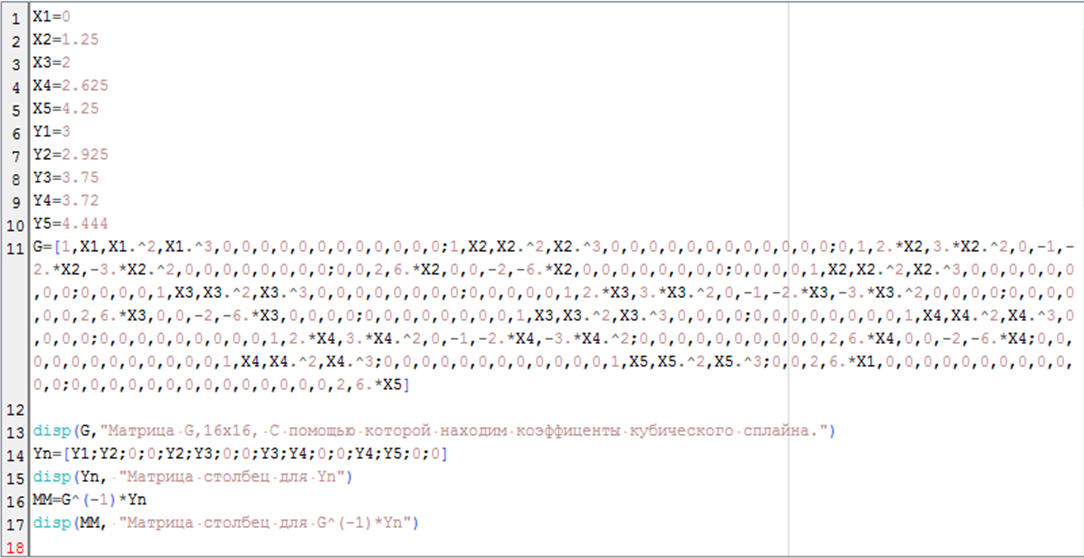
\includegraphics[width=0.9\linewidth]{2,1.PNG}} \\
\caption{Первая часть скрипта для вычисления сплайна}
\end{figure}

\begin{figure}[H]
\center{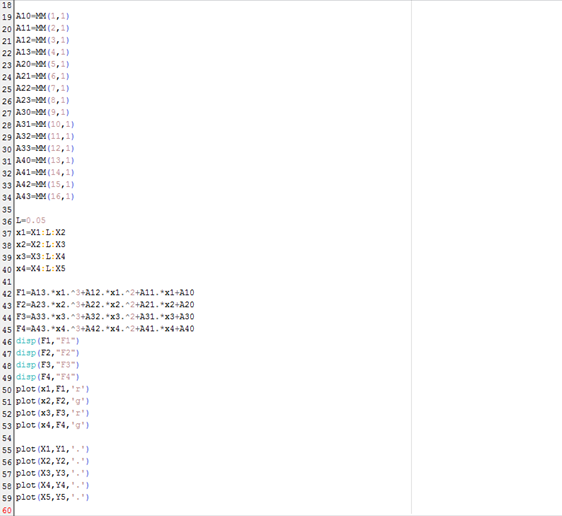
\includegraphics[width=0.9\linewidth]{2,2.PNG}} \\
\caption{Вторая часть скрипта для вычисления сплайна}
\end{figure}

\begin{figure}[H]
\center{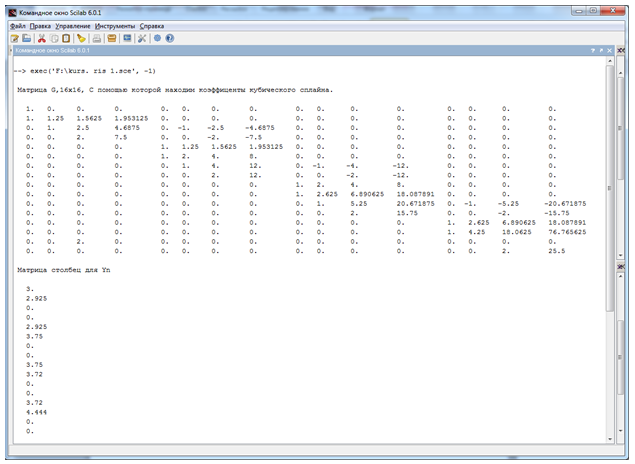
\includegraphics[width=0.9\linewidth]{2,3.PNG}} \\
\caption{Матрица }
\end{figure}

\begin{figure}[H]
\center{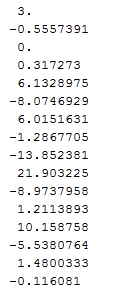
\includegraphics[width=0.3\linewidth]{2,4.PNG}} \\
\caption{Значения для коэффицентов $A_{ij}$}
\end{figure}

Окончательные уравнения сплайна
$$F_1=0,317x^3+0x^2-0,556x+3$$
$$F_2=-1,287x^3+6,015x^2-8,075x+6,133$$
$$F_3=1,211x^3-8,974x^2+21,903x-13,852$$
$$F_4=-0,116x^3+1,48x^2-5,538x+10,159$$

\begin{figure}[H]
\center{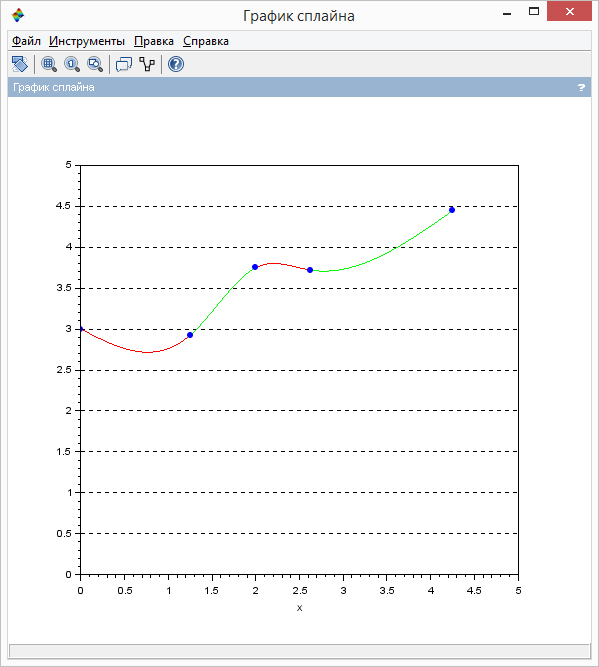
\includegraphics[width=0.8\linewidth]{2,5.PNG}} \\
\caption{Построение кубического сплайна}
\end{figure}

\subsection{Нахождение значения функции в тоxке Х=2,1}
Найдём значение функции в точке х=2,1
Подставим х=2,1 в полином данного промежумка 
$$F_3=1,211x^3-8,974x^2+21,903x-13,852$$
$$y_{(x=2,1)}=3,784$$

\newpage

\subsection{Оценка погрешности интерополяции в точке х=3.1}

 Оценка погрешности интерполяции Эрмитовыми
кубическими сплайнами проводится после получения четвёртой производной функции. Далее вычисляем h -- из координаты х точки в которой вычисляется погрешность вычитаем координату ближайшей к ней точки $x_4=2.625$. После чего подставляем значения в формулу $P=\frac{1}{384}h^4|f^{IV}(x)|$
$$F'_1=\frac{Y_2-Y_1}{X_2-X_1}=-0.06$$
$$F'_2=\frac{Y_3-Y_2}{X_3-X_2}=1.1$$
$$F'_3=\frac{Y_4-Y_3}{X_4-X_3}=-0.048$$
$$F'_4=\frac{Y_5-Y_4}{X_5-X_4}=0.4455385$$
\
$$F''_1=\frac{F'_2-F'_1}{X_3-X_1}=0.58$$
$$F''_2=\frac{F'_3-F'_2}{X_4-X_2}=-0.8349091$$
$$F''_3=\frac{F'_4-F'_3}{X_5-X_3}=0.2193504$$ 
\
$$F'''_1=\frac{F'_2-F'_1}{X_4-X_1}=-0.539013$$
$$F'''_2=\frac{F'_3-F'_2}{X_5-X_2}= 0.3514198$$ 
\
$$F^{IV}=\frac{F'_2-F'_1}{X_5-X_1}=0.2095136$$ 
\
$$h=X-X_4=0.475$$
\
$$P=\frac{1}{384}h^4|f^{IV}(x)|= 0.0000278=278 \cdot 10^{-7}$$ 

Вычисления оценки погрешности интерполяции Эрмитовыми
кубическими сплайнами, и необходимая для этого четвёртая производная функция, находились при помощи программы "Scilab" . Для удобства написания и редактирования во встроенном в программу текстовом редакторе "SciNotes" был написан скрипт. Он является продолжением скрипта нахождения собственно сплайна.  По нему найдено решение. 
\\ \\
\begin{figure}[H]
\center{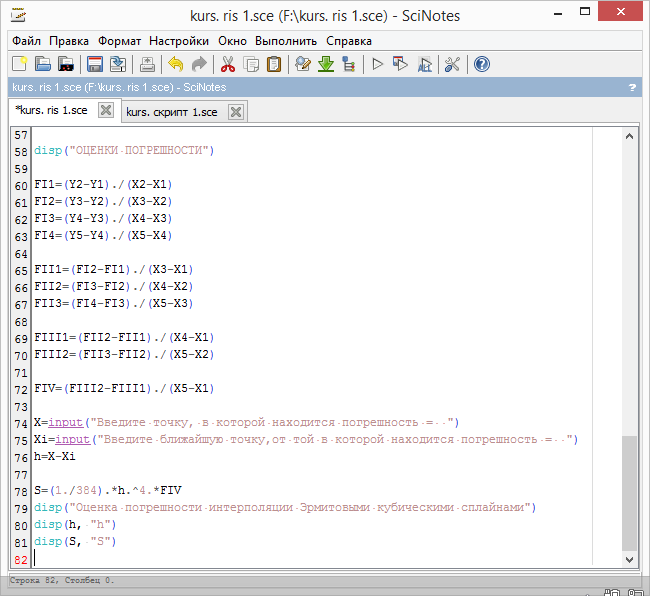
\includegraphics[width=0.9\linewidth]{2,6.PNG}} \\
\caption{Продолжение скрипта.Оценка погрешности}
\end{figure}


\begin{figure}[H]
\center{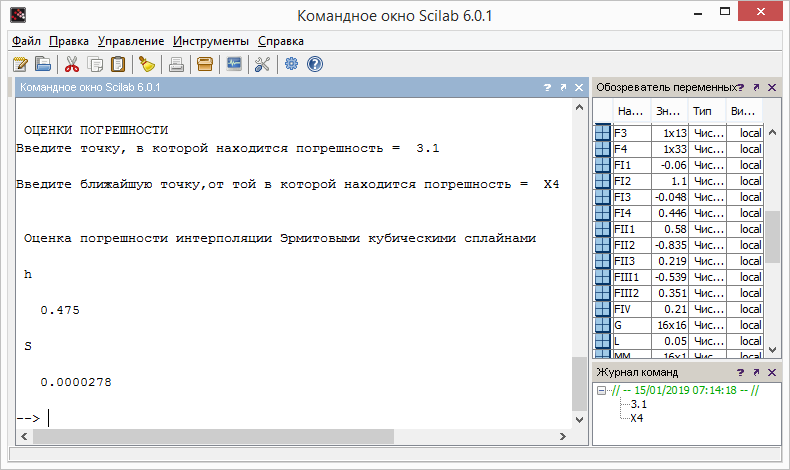
\includegraphics[width=0.9\linewidth]{2,7.PNG}} \\
\caption{Командное окно. Оценка погрешности}
\end{figure}

\newpage

%%%%%%%%%%%%%%%%%%%%%%%%%%%%%%%%%%%%%%%%%%%%%%%%%%%%%%%%%%%%%%
\section{Оптимальное распределение неоднородных ресурсов.}


Решить задачу оптимального распределения неоднородных ресурсов. \\


Пусть в распоряжении завода железобетонных изделий (ЖБИ) имеется m видов сырья (песок, щебень, цемент) в обёмах $a_i$. Требуется произвести продукцию n видов. Дана трёхнологическая норма $c_{ij}$ потребления отдельного i-го вида. Известна прибыль $П_i$, получаемая от выпуска единицы продукции j-го вида. Требуется определить, какую продукциюи  в каком количестве должен производить завод ЖБИ, чтобы получить максимальную прибыль.

%%%
\begin{table}[h]

\caption{\label{1} Задание согласно варианту:  }
\renewcommand{\tabcolsep}{0.5cm}
\begin{center}
\begin{tabular}{|c|c|c|c|c|c|c|c|c|c|c|c|}
\hline 
Используемые ресурсы &\multicolumn{4}{|c|}{Изготавливаемые изделия} & Наличие\\
ресурсы $a_i$ & $U_1$ & $U_2$ & $U_3$ & $U_4$ & ресурсов $a_i$\\

\hline
  Песок          & 3  & 7  & 6  & 7  & 16  \\
  Щебень         & 4  & 5  & 5  & 1  & 12  \\
  Цемент         & 4  & 4  & 9  & 8  & 35  \\
  Прибыль, П$_j$ & 35 & 45 & 36 & 28 &   \\
 \hline
\end{tabular}
\end{center}
\end{table} 

 Для нахождения целочисленных значений в решении задачи на распределение неоднородных ресурсов воспользуемся функчией linpro доступной при установке пакета  lpsolve.
Все значения технологических норм на материалы запишем в виде матрицы а;
ограничения на сырьё -- вектор b;  вектор прибыли - с; также нужно ввести
вектор e, определяющий оператор отношения для ограничений $(\leq  =  \geq)$;
vlb – вектор, задающий нижнюю границу переменных;
xint – вектор, задающий ограничение на переменные, в множестве целых чисел.



\begin{figure}[H]
\center{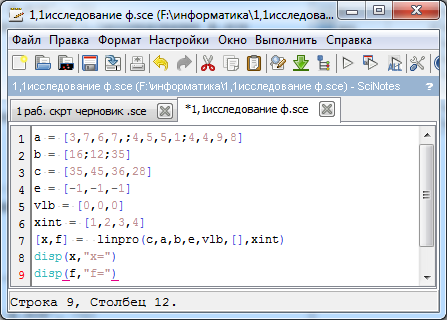
\includegraphics[width=0.7\linewidth]{3,1.png}} \\
\caption{расчёт распределения неоднородных ресурсов}
\end{figure}


х=[3,0,0,0] 


f=105\\

Таким образом было выяснено, что предприятие получет максимальную прибыль при производстве трёх изделий U1.  И эта прибыль составит 105 условных единиц.

\newpage

\section{Вывод.}

В данной работе были получены навыки владения математического пакета  "Scilab" . Были изучены методы исследование функций и сплайнов, построения графиков и распределение ресурсов.Решена задача по построению и изучению функции. Построен кубический сплайн, и оценена погрешность интерополяции в одной из его точек. А так же рассмотрены методы распределения неоднородных ресурсов.




\newpage
\section{Список литературы.}

1. Ю.С. Завьялов. Методы сплайн-функций. М.Наука, 1980.

2. Introduction in SciLab

3. Андриевский А.Б., Андриевский Б.Р.,Капитонов А.А.Решение инженерных задач в SCILAB

4. Калиткин Численные методы. М., Мир. 1980.

5.smath studio user’s manual






\end{document}














